%==============================================================================
% Sjabloon onderzoeksvoorstel bachproef
%==============================================================================
% Gebaseerd op document class `hogent-article'
% zie <https://github.com/HoGentTIN/latex-hogent-article>

% Voor een voorstel in het Engels: voeg de documentclass-optie [english] toe.
% Let op: kan enkel na toestemming van de bachelorproefcoördinator!
\documentclass{hogent-article}

% Invoegen bibliografiebestand
\addbibresource{voorstel.bib}

% Informatie over de opleiding, het vak en soort opdracht
\studyprogramme{Professionele bachelor toegepaste informatica}
\course{Bachelorproef}
\assignmenttype{Onderzoeksvoorstel}
% Voor een voorstel in het Engels, haal de volgende 3 regels uit commentaar
% \studyprogramme{Bachelor of applied information technology}
% \course{Bachelor thesis}
% \assignmenttype{Research proposal}

\academicyear{2023-2024} % TODO: pas het academiejaar aan

% TODO: Werktitel
\title{Optimalisatie van educatief gebruik: beperking en flexibele activering van E-commerce platforms en sociale media in het onderwijs}

% TODO: Studentnaam en emailadres invullen
\author{Steph Schevernels}
\email{Steph.schevernels@student.hogent.be}

% TODO: Medestudent
% Gaat het om een bachelorproef in samenwerking met een student in een andere
% opleiding? Geef dan de naam en emailadres hier
% \author{Yasmine Alaoui (naam opleiding)}
% \email{yasmine.alaoui@student.hogent.be}

% TODO: Geef de co-promotor op
\supervisor[Co-promotor]{Peter Vandebeek(IÑIGO, \href{mailto:peter.vandebeek@inigo-ignatiaansescholen.be}{peter.vandebeek@inigo-ignatiaansescholen.be})}

% Binnen welke specialisatierichting uit 3TI situeert dit onderzoek zich?
% Kies uit deze lijst:
%
% - Mobile \& Enterprise development
% - AI \& Data Engineering
% - Functional \& Business Analysis
% - System \& Network Administrator
% - Mainframe Expert
% - Als het onderzoek niet past binnen een van deze domeinen specifieer je deze
%   zelf
%
\specialisation{System \& Network Administrator}
\keywords{Digitale Focusmanagement, Educatieve Technologie , Leerkrachtelijke Autorisatie }

\begin{document}

\begin{abstract}
   Deze bachelorproef onderzoekt de optimalisatie van educatief gebruik: beperking en flexibele activering van E-commerce Platforms en sociale media in het onderwijs. Ook vergelijkt het welke methode de balans tussen gebruiksgemak, algemene kosten en functionaliteiten voor het beheren van toegang tot E-commerce en social media platforms in het onderwijs vormt, met als doel de afleiding te minimaliseren en educatief gebruik te optimaliseren. De motivatie voor dit onderzoek ligt in de groeiende uitdagingen waarmee het onderwijs geconfronteerd wordt bij het beheren van een gebalanceerde en gecontroleerde toegang tot E-commerce en social media platforms. In een vergelijkende proof-of-concept werden zowel zeven software-methoden vergeleken en geïmplementeerd als een proxy methode uitgewerkt. De verwachte conclusie van dit onderzoek betrekt één specifieke methode of softwareprogramma dat volledig voldoet aan de gestelde criteria en de vereisten van de casus. Hieruit kan geconcludeerd worden dat er een passende methode nodig is om centraal beheer van de websites te manifesteren, zodat leerlingen flexibele toegang hebben tot websites die niet van toepassing zijn tijdens de schooluren.
\end{abstract}

\tableofcontents

% De hoofdtekst van het voorstel zit in een apart bestand, zodat het makkelijk
% kan opgenomen worden in de bijlagen van de bachelorproef zelf.
%---------- Inleiding ---------------------------------------------------------

\section{Introductie}%
\label{sec:introductie}
In een tijdsperiode waarin digitale technologie niet meer weg te denken is, ondergaat het onderwijs een zware transformatie. Hierin bieden E-commerce platforms en sociale media in een educatieve omgeving verscheidene mogelijkheden om het leerproces te verreiken en studenten voor te bereiden op uitdagingen in de moderne samenleving. Echter kunnen deze platformen ook voor heel veel afleiding zorgen. Hierdoor is er nood aan digitale middelen om deze afleiding tijdens de lessen tegen te gaan. 

Deze studie richt zich op de optimalisatie van educatief gebruik door middelen van gerichte beperkingen en flexibele activering van E-commerce en sociale media platforms. Deze diepgaande studie richt zich op verscheidene methoden die momenteel worden toegepast in het onderwijs om zo een evenwicht te vinden tussen de toegang en het minimaliseren van de afleiding betrekkend tot waardevolle digitale hulpmiddelen. Dit gaande van zowel lagere als middelbare scholen. 

In deze bachelorproef wordt volgende onderzoeksvraag gesteld:
\begin{itemize}
    \item Welke methode vormt de balans tussen gebruiksgemak, algemene kosten en functionaliteiten voor het beheren van toegang tot E-commerce en social media platforms in het onderwijs, met als doel de afleiding te minimaliseren en educatief gebruik te optimaliseren? 
\end{itemize}


%---------- Stand van zaken ---------------------------------------------------

\section{Literatuurstudie}%
\label{sec:state-of-the-art}
\subsection{Educatieve Technologie in de 21e Eeuw}
In de 21e eeuw is technologie niet meer weg te denken uit de samenleving. Maar dit is ook zo in scholen. Wanneer er wordt ingezoomd op de leeromgeving waar leerlingen en studenten zich bevinden, zijn er veel veranderingen opgetreden. ``Klaslokalen over de hele wereld worden technologisch steeds geavanceerder. Een groeiende trend is dat scholen elke leerling een persoonlijke laptop of tablet ter beschikking stellen, zowel voor gebruik in de klas als thuis.'' \textcite{HALL2021101957} Dit alles is in een versneld temp geëvolueerd na de COVID-pandemie. Waardoor scholen ook in een versneld tempo moest schakelen om deze vereisten op te zetten in hun gebouwen, denk maar aan meer stopcontacten, beter internet, middelen voor arme gezinnen.\newline
Vervolgens moesten de scholen hun leerpakketten ook aanpassen zodat leerlingen meer met de computer konden werken tijdens de lessen. Hierdoor waren leerkrachten in staat tot overschakeling van zelfstandiger onderwijs. Anderzijds toont onderzoek aan dat leerlingen sneller afgeleid zijn bij het gebruik van laptops en tablets in de les. \textcite{deng2020laptops} Hierdoor was er dus nood aan verscheidene methoden of technologieën die in staat zijn de leerlingen toch bij de les te houden. Deze technologieën worden ook wel Classroom management software (CMS) genoemd.

\subsection{Wat is Classroom management software}
``Classroom management software (CMS) stelt leerkrachten in staat om de apparaat activiteit van leerlingen te bekijken, controleren en beheren. De software biedt leerkrachten een gecentraliseerd overzicht van alle leerlingen hun scherm in de klas en de mogelijkheid om niet-gerelateerde tabbladen te sluiten, schermen te vergrendelen en meer.'' \autocite{ClassroomManagement} 
Voorbeelden hiervan zijn: LanSchool, Netop Vision, Securly, Lightspeed Classroom Management en GOGuardian Teacher. 
Kenmerkend aan deze software is de verscheidene functies die gebruikers hiermee kunnen verwezenlijken
\begin{itemize}
    \item Beheer alle lessen vanaf de startpagina
    \item Creëren van virtuele groepen 
    \item Stuur expresberichten naar de schermen van leerlingen hun apparaten 
    \item Push links naar een leerling of de hele klas
    \item Ontvang updates over de status van studenten 
    \item Tel webregels in om specifieke websites te beperken
    \item Onderzoek de browsergeschiedenis van leerlingen 
    \item Bekijk schermen van de hele klas in één keer of zoom in op een afzonderlijk scherm
    \item Registreer de activiteit op het scherm van een leerling
    \newline
    \autocite{Lightspeed}
\end{itemize}

\subsection{Beveiliging en privacy van Classroom management software}
Doordat deze programma's verschillende schermen kunnen weergeven van elke leerling, is het uiteraard belangrijk dat deze programma's goed beveiligd worden. Ook moeten er duidelijke regels opgesteld worden voor de leerkrachten. Denk maar aan het gebruik van deze programma's buiten de school zelf. Ook worden de virtuele klassen versleuteld zodat geen enkel persoon kan meekijken tijdens de les. Vooraleer leerkrachten toegang mogen verschaffen tot de controle van ieders scherm moeten de leerlingen het privacybeleid van de school goedkeuren. Wanneer ze dit niet goedkeuren mag de leerkracht geen gebruik maken van het programma bij de desbetreffende leerling. \autocite{privacy}


\subsection{Gebruik van E-commerce en social media platforms tijdens de lessen}
Onderzoek toont aan dat sociale media in vele gevallen ook positief kan zijn in het onderwijs, zowel voor leerlingen als leerkrachten. Het gebruik ervan kan dienen als direct communicatiemiddel tussen leerkracht en student, waar sociale media wordt ingezet om aankondigingen en updates te plaatsen om zo discussies in vermeiden. 
Vervolgens kan de studentenbetrokkenheid verhoogd worden dankzij social media tools. Naast de stimulatie van leerlingen zorgen deze platforms ook voor actieve deelname aan het vormgeven van de eigen leerervaring. Hierdoor kunnen studenten zich comfortabel uiten, samenwerken en waardevolle leermiddelen delen en raadplegen, onafhankelijk van tijd en plaats. \newline
Tot slot wordt er in de studie nog een laatste aspect besproken, namelijk sociale media als samenwerkingsplatform. Hierbij bevordert de samenwerking tussen leerlingen, leerkrachten en andere betrokkenen door kennis uit te wisselen. Zo kunnen samenwerkingstools zoals 'Google Docs' makkelijker worden gedeeld en kan ieder zijn steentje bijdragen door gebruik te maken van gedeelde inhoud. Op deze manier wordt de samenwerking tussen leerlingen verbeterd. \newline
De voordelen van sociale media leggen de basis bij het gebruik van E-commerce platforms tijdens de lessen, waarbij gevaarlijke en foute verkoopsites worden aangekaart om leerlingen te waarschuwen voor frauduleuze websites. Wat resulteert in oplettende studenten die zich ervan bewust zijn dat niet elke reclame betrouwbaar is. Hierdoor zullen jongeren meer nadenken vooraleer ze een bestelling plaatsen op een onbekende website.   \autocite{benefitsofsocialmedia} \autocite{onlinefraude}


%---------- Methodologie ------------------------------------------------------
\section{Methodologie}%
\label{sec:methodologie}
Om het onderzoek te beginnen, wordt er vooreerst gestart met een literatuurstudie. De doelstelling van deze literatuurstudie is het verkennen van de bestaande literatuur en software over de verschillende methoden voor het flexibel activeren van E-commerce en social media platforms in de huidige onderwijsomgeving. De aanpak die hiervoor gebruikt zal worden is grondig onderzoek van wetenschappelijke artikelen, rapporten en andere relevante bronnen die van toepassing zijn hierop om inzicht te krijgen in de verschillende methoden, hun effectiviteit en kost. \newline

Na deze literatuurstudie wordt er gestart aan de tweede fase, wat het uitvoeren van een vergelijkende proof-of-concept is. Het doel van deze aanpak is het opzetten van een testomgeving waarbij een klasomgeving wordt nagebootst. Hierdoor kunnen verscheidene opties getest worden waarvan de beste wordt gebruikt als conclusie. Een goede testomgeving bestaat uit 3 eigenschappen, namelijk reproduceerbaarheid, repliceerbaarheid en herbruikbaarheid. Deze 3 eigenschappen worden uitdrukkelijk gevolgd tijdens de opzet van de testomgeving doorheen dit onderzoek. De eerste stap van de proof-of-concept is het opzetten van de testomgeving waar in gewerkt wordt. Om deze omgeving op te zetten is er uiteraard apparatuur nodig. Doordat dit een testomgeving is wordt er gebruik gemaakt van virtuele machines en geen echte computers, wat de kosten ook drukt. De virtuele machines draaien op één computer met Virtualbox software met als besturingssysteem Windows 10. In deze fase wordt tevens voor elke machine een uniek account aangemaakt, zodat de leerkracht onderscheid maken tussen zichzelf en de leerlingen en bijgevolg rechten per account kunnen worden toegewezen. Er wordt gekozen voor 4 virtuele machines waarvan 3 voor de leerlingen en 1 voor de leerkracht computer. Omdat deze stap zich alleen beperkt tot het installeren van virtuele machines en het aanmaken hiervan, wordt er een tijdspanne worden gekozen van 2 weken. Tijdens deze 2 weken worden deze machines ook met elkaar gekoppeld op één zelfde netwerk zodat deze met elkaar kunnen communiceren. \newline

Na het opzetten van de virtuele machines kan de verschillende software geïnstalleerd worden om nadien uitgebreid te testen. Hiervoor wordt er gestart met Classroom Management Software waarbij LanSchool, Netop Vision, Securly, Lightspeed Classroom Management en GOGuardian Teacher vergeleken worden. Daarnaast is het ook een mogelijkheid om via proxy-server dezelfde taken uit te voeren als Classroom Management Software. Dit wordt in deze stap uitgebreid worden uitgevoerd en getest. Omdat deze stap tijdrovend is voor elke installatie te vergelijken en te installeren wordt er gekozen voor een tijdspanne van 4 tot 5 weken.  \newline

Na het installeren van verscheidene tools wordt er duidelijk welke in aanmerking komt voor gebruik. Hierdoor kan er aan de tweede eigenschap van proof-of-concept gewerkt worden, namelijk repliceerbaarheid. Hierbij wordt de volledige testopstelling van gekozen tools geautomatiseerd, zodat deze testomgeving repliceerbaar is. Voor deze stap wordt er geoogd op een tijdspanne van 4 weken. \newline

Tot slot wordt de overige tijd gebruikt voor de derde eigenschap namelijk herbruikbaarheid. Dit is de laatste fase van onze methodologie waarbij vergelijkbare varianten van deze testopstelling in acht worden genomen. Hierbij worden de verschillende automatisaties uitgerold, zodat er onderling kan vergeleken worden. \newline

\begin{figure}[h]
    \centering
    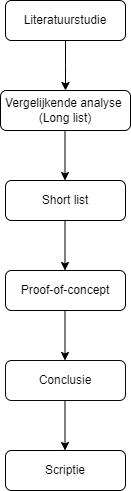
\includegraphics[width=.3\linewidth]{Flowchart.png}
    \caption{Flowchart methodologie.}
    \label{fig:Flowchart}
\end{figure}


%---------- Verwachte resultaten ----------------------------------------------
\section{Verwacht resultaat, conclusie}%
\label{sec:verwachte_resultaten}

Na het voltooien van de vergelijkende proof-of-concept wordt er verwacht dat de Classroom Management software of proxy-serveroplossing zich als effectief resulteert, zodat de E-commerce en sociale media platforms beperkt en flexibel geactiveerd worden in een klas. De keuze voor de meest geschikte oplossing hangt af van verscheidene vereisten die de balans vormen tussen gebruiksgemak, algemene kosten en functionaliteiten. De conclusie wordt gevormd door de concrete aanbevelingen voor het flexibel beheren van E-commerce en social media platforms in een onderwijsomgeving, met als doel minimalisatie van afleiding bij studenten tijdens de schooluren.

\printbibliography[heading=bibintoc]

\end{document}